%\section{Parallel program profiler analysis}
%After the parallel program implementation, another round of profiling using \code{cProfile} was conducted. This was done on the initial testing laptop,
%with 4 workers, on the same dataset as the first round of profiling. The results from the main process that orchestrates the other processes and aggregates their results can be
%found in \ref{fig:parallel_profiler_main}. The results from two of the workers can be found in figure \ref{fig:parallel_profiler_w1} and figure \ref{fig:parallel_profiler_w2}.
%
%For the main process, it is apparent that \code{post\_process\_parallel}, the function that makes the trade ID:s unique after the parallel worker processes have finished
%executing, adds non-negligible overhead. \code{aggregate\_result} contains the code that creates the other processes and waits for these to produce their partial results,
%aggregating them as they are produced. This code takes up 84\% of the total time, while the remaining 16\% of the code is effectively overhead.
%In addtion, as mentioned in section \ref{section:sequential_profiler} as a possibility, \code{\_prepare} is called for each
%worker process, resulting in extra overhead. It is conceivable that these sources of overhead are less noticable when processing a larger dataset, as the effects of
%the functions that are called only one time take up a smaller amount of the total running time if the dataset contains a larger number of rows.
%
%For the worker processes, the results are similar to the results from profiling the sequential program in section \ref{section:sequential_profiler}, but with lower
%\code{cumtime} values. This is expected due to the lower number of rows per worker. The same functions as in the sequential program are responsible for the largest
%portion of the running time, \code{process\_record}, \code{post\_process\_record}, \code{consume\_record}, and \code{\_prepare}.
%
%\begin{figure}[ht]
  %\lstinputlisting[basicstyle=\tiny]{figures/profiling_parallel_19_may_main.txt}
  %\caption{Main process in parallel program \code{cProfile} output}
  %\label{fig:parallel_profiler_main}
%\end{figure}
%\clearpage
%
%\begin{figure}[ht]
  %\lstinputlisting[basicstyle=\tiny]{figures/profiling_parallel_19_may_31147.txt}
  %\caption{Worker 1 in parallel program \code{cProfile} output}
  %\label{fig:parallel_profiler_w1}
%\end{figure}
%\clearpage

%\begin{figure}[ht]
  %\lstinputlisting[basicstyle=\tiny]{figures/profiling_parallel_19_may_31148.txt}
  %\caption{Worker 2 in parallel program \code{cProfile} output}
  %\label{fig:parallel_profiler_w2}
%\end{figure}
%\clearpage


\section{Transformation benchmarks}
The benchmarks for the experiments are outlined below. For each dataset, the results consist of a table containing
speedup, real time, user time, system time, and memory usage for each worker number. The standard deviation is represented
as a value following the $\pm$ sign. The value S in worker column signifies the original sequential program, while 1 is the
parallel program with a single worker. In addition to the tables, the real time, speedup, and memory usage are illustrated
using plots in order to visually demonstrate how the values change with the number of workers. In the plots for real time
and memory usage, the standard deviation is illustrated using black bars above and below each data point\footnote{
The standard deviation is shown for all plots of real time and memory usage, but it may be too small to be seen for some of the plots.}.

\section{Benchmark tables}
\subsection{Tiny dataset benchmark table}
The benchmark for the tiny dataset can be found in figure \ref{fig:dataset_1_table}.
The table displays the number of workers, the speedup (sequential run real time divided by real time), real time,
user time, system time, and memory usage. The standard deviation is displayed with a value following the $\pm$ sign.

\begin{figure}[ht]
\centering
\resizebox{\linewidth}{!}{%
\begin{tabular}{|c|c|c|c|c|c|}%
  \hline
  \bfseries Workers & \bfseries Speedup & \bfseries Real (s) & \bfseries User (s) & \bfseries System (s) & \bfseries Memory usage (MB)
  \csvreader[respect all,head to column names]{figures/dataset_1/dataset_1_table.csv}{workers=\w,speedup=\spd,real=\r,user=\u,system=\s,memory_usage_mb=\m}
  {\\\hline \w & \spd & \r & \u & \s & \m}
  \\ \hline
\end{tabular}}
\caption[Tiny dataset benchmark table.]{Tiny dataset benchmark table. The table displays the number of workers, the speedup (sequential run real time divided by real time), real time,
user time, system time, and memory usage. The standard deviation is displayed with a value following the $\pm$ sign.}
\label{fig:dataset_1_table}
\end{figure}

\subsection{Small dataset benchmark table}
The benchmark for the small dataset can be found in figure \ref{fig:dataset_2_table}.
The table displays the number of workers, the speedup (sequential run real time divided by real time), real time,
user time, system time, and memory usage. The standard deviation is displayed with a value following the $\pm$ sign.

\begin{figure}[ht]
\centering
\resizebox{\linewidth}{!}{%
\begin{tabular}{|c|c|c|c|c|c|}%
  \hline
  \bfseries Workers & \bfseries Speedup & \bfseries Real (s) & \bfseries User (s) & \bfseries System (s) & \bfseries Memory usage (MB)
  \csvreader[respect all,head to column names]{figures/dataset_2/dataset_2_table.csv}{workers=\w,speedup=\spd,real=\r,user=\u,system=\s,memory_usage_mb=\m}
  {\\\hline \w & \spd & \r & \u & \s & \m}
  \\ \hline
\end{tabular}}
\caption[Small dataset benchmark table.]{Small dataset benchmark table. The table displays the number of workers, the speedup (sequential run real time divided by real time), real time,
user time, system time, and memory usage. The standard deviation is displayed with a value following the $\pm$ sign.}
\label{fig:dataset_2_table}
\end{figure}

\subsection{Medium dataset benchmark table}
The benchmark for the medium dataset can be found in figure \ref{fig:dataset_3_table}.
The table displays the number of workers, the speedup (sequential run real time divided by real time), real time,
user time, system time, and memory usage. The standard deviation is displayed with a value following the $\pm$ sign.

\begin{figure}[ht]
\centering
\resizebox{\linewidth}{!}{%
\begin{tabular}{|c|c|c|c|c|c|}%
  \hline
  \bfseries Workers & \bfseries Speedup & \bfseries Real (s) & \bfseries User (s) & \bfseries System (s) & \bfseries Memory usage (MB)
  \csvreader[respect all,head to column names]{figures/dataset_3/dataset_3_table.csv}{workers=\w,speedup=\spd,real=\r,user=\u,system=\s,memory_usage_mb=\m}
  {\\\hline \w & \spd & \r & \u & \s & \m}
  \\ \hline
\end{tabular}}
\caption[Medium dataset benchmark table.]{Medium dataset benchmark table. The table displays the number of workers, the speedup (sequential run real time divided by real time), real time,
user time, system time, and memory usage. The standard deviation is displayed with a value following the $\pm$ sign.}
\label{fig:dataset_3_table}
\end{figure}

%\subsection{Large dataset benchmark table}
%The benchmark for the small dataset can be found in figure \ref{fig:dataset_4_table}.
%The table displays the number of workers, the speedup (sequential run real time divided by real time), real time,
%user time, system time, and memory usage. The standard deviation is displayed with a value following the $\pm$ sign.
%
%\begin{figure}[ht]
%\centering
%\resizebox{\linewidth}{!}{%
%\begin{tabular}{|c|c|c|c|c|c|}%
  %\hline
  %\bfseries Workers & \bfseries Speedup & \bfseries Real (s) & \bfseries User (s) & \bfseries System (s) & \bfseries Memory usage (MB)
  %\csvreader[respect all,head to column names]{figures/dataset_4/dataset_4_table.csv}{workers=\w,speedup=\spd,real=\r,user=\u,system=\s,memory_usage_mb=\m}
  %{\\\hline \w & \spd & \r & \u & \s & \m}
  %\\ \hline
%\end{tabular}}
%\caption[Large dataset benchmark table.]{Large dataset benchmark table. The table displays the number of workers, the speedup (sequential run real time divided by real time), real time,
%user time, system time, and memory usage. The standard deviation is displayed with a value following the $\pm$ sign.}
%\label{fig:dataset_4_table}
%\end{figure}

\section{Execution time}

\subsection{Tiny dataset execution time}
The real execution time for the tiny dataset can be found in figure \ref{fig:dataset_1_real_time}.
The X axis shows the number of workers, where 0 signifies the sequential program run.
The Y axis shows the real execution time for each worker value. The standard deviation is displayed with black bars around each data point. Real time
increases as number of workers increase. The data points at 10 and 13 workers show high standard deviation.
\begin{figure}[ht]
  \centering
  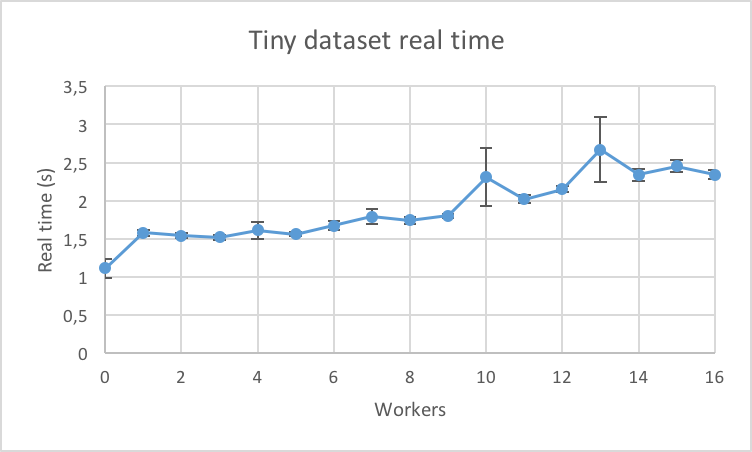
\includegraphics[width=120mm]{figures/dataset_1/dataset_1_real_time.png}
  \caption[Real time plot for the tiny dataset.]{Real time plot for the tiny dataset. The X axis shows the number of workers, where 0 signifies the sequential program run.
  The Y axis shows the real execution time for each worker value. The standard deviation is displayed with black bars around each data point. Real time
  increases as number of workers increase. The data points at 10 and 13 workers show high standard deviation.}
  \label{fig:dataset_1_real_time}
\end{figure}

\subsection{Small dataset execution time}
The real execution time for the small dataset can be found in figure \ref{fig:dataset_2_real_time}.
The X axis shows the number of workers, where 0 signifies the sequential program run.
The Y axis shows the real execution time for each worker value. The standard deviation is displayed with black bars around each data point. The real time
decreases with each added worker up to 8 workers, where it evens out. The decrease in real time for each added worker becomes smaller as the number increases.
\begin{figure}[ht]
  \centering
  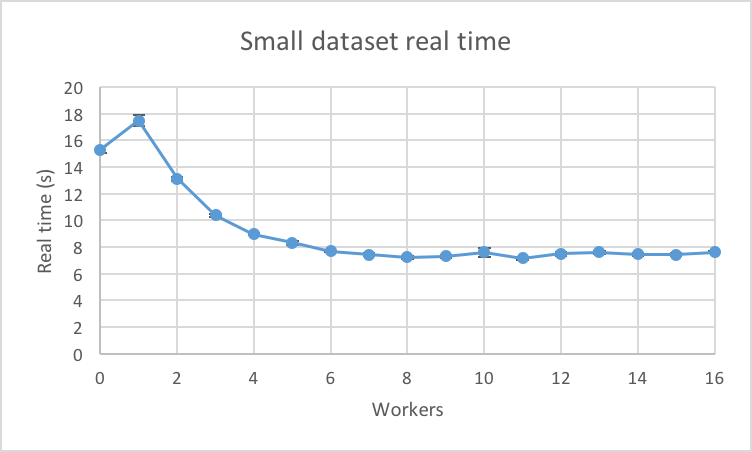
\includegraphics[width=120mm]{figures/dataset_2/dataset_2_real_time.png}
  \caption[Real time plot for the small dataset.]{Real time plot for the small dataset. The X axis shows the number of workers, where 0 signifies the sequential program run.
  The Y axis shows the real execution time for each worker value. The standard deviation is displayed with black bars around each data point. The real time
  decreases with each added worker up to 8 workers, where it evens out. The decrease in real time for each added worker becomes smaller as the number increases.}
  \label{fig:dataset_2_real_time}
\end{figure}

\subsection{Medium dataset execution time}
The real execution time for the medium dataset can be found in figure \ref{fig:dataset_3_real_time}.
The X axis shows the number of workers, where 0 signifies the sequential program run.
The Y axis shows the real execution time for each worker value. The standard deviation is displayed with black bars around each data point. The real time
decreases with each added worker up to 8 workers, where it evens out. The decrease in real time for each added worker becomes smaller as the number increases.
\begin{figure}[ht]
  \centering
  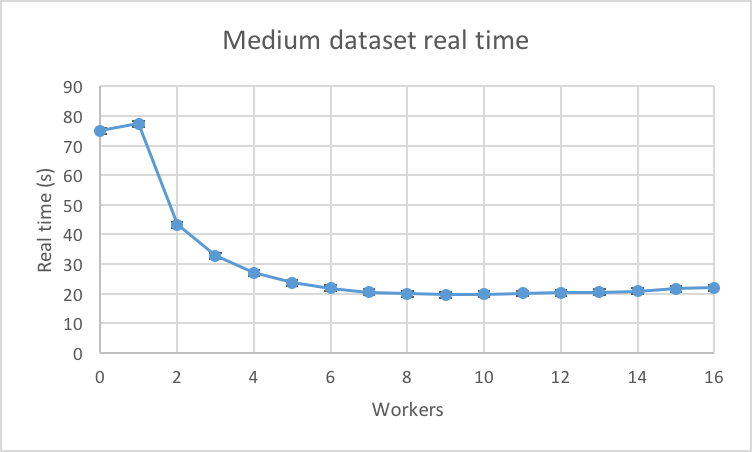
\includegraphics[width=120mm]{figures/dataset_3/dataset_3_real_time.png}
  \caption[Real time plot for the medium dataset.]{Real time plot for the medium dataset. The X axis shows the number of workers, where 0 signifies the sequential program run.
  The Y axis shows the real execution time for each worker value. The standard deviation is displayed with black bars around each data point. The real time
  decreases with each added worker up to 8 workers, where it evens out. The decrease in real time for each added worker becomes smaller as the number increases.}
  \label{fig:dataset_3_real_time}
\end{figure}

%\subsection{Large dataset execution time}
%The real execution time for the small dataset can be found in figure \ref{fig:dataset_4_real_time}.
%The X axis shows the number of workers, where 0 signifies the sequential program run.
%The Y axis shows the real execution time for each worker value. The standard deviation is displayed with black bars around each data point. The real time
%decreases with each added worker up to 12 workers, where it evens out. The decrease in real time for each added worker becomes smaller as the number increases.
%\begin{figure}[ht]
  %\centering
  %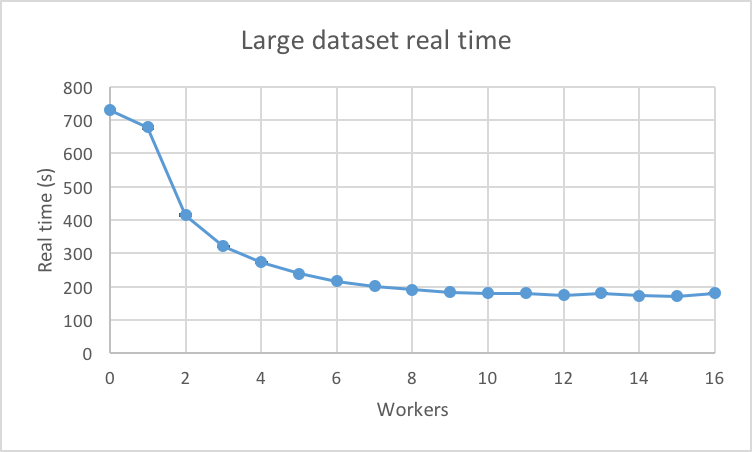
\includegraphics[width=120mm]{figures/dataset_4/dataset_4_real_time.png}
  %\caption[Real time plot for the large dataset.]{Real time plot for the large dataset. The X axis shows the number of workers, where 0 signifies the sequential program run.
  %The Y axis shows the real execution time for each worker value. The standard deviation is displayed with black bars around each data point. The real time
  %decreases with each added worker up to 12 workers, where it evens out. The decrease in real time for each added worker becomes smaller as the number increases.}
  %\label{fig:dataset_4_real_time}
%\end{figure}

\section{Speedup}

\subsection{Tiny dataset speedup}
The speedup for the tiny dataset can be found in figure \ref{fig:dataset_1_speedup}.
The X axis shows the number of workers, and the Y axis shows a scalar value signifying the speedup as
``number of times faster than sequential execution''. Speedup decreases with each added worker, down to about half the speed of the sequential execution.
\begin{figure}[ht]
  \centering
  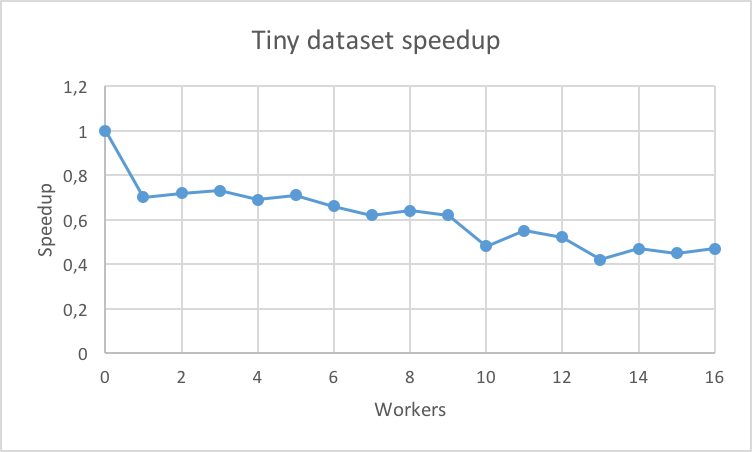
\includegraphics[width=120mm]{figures/dataset_1/dataset_1_speedup.png}
  \caption[Speedup plot for tiny dataset.]{Speedup plot for the tiny dataset. The X axis shows the number of workers, and the Y axis shows a scalar value signifying the speedup as
  ``number of times faster than sequential execution''. Speedup decreases with each added worker, down to about half the speed of the sequential execution.}
  \label{fig:dataset_1_speedup}
\end{figure}

\subsection{Small dataset speedup}
The speedup for the small dataset can be found in figure \ref{fig:dataset_2_speedup}.
The X axis shows the number of workers, and the Y axis shows a scalar value signifying the speedup as
``number of times faster than sequential execution''. Speedup increases with each worker, evening out around 8 workers and 2.1X speedup.
\begin{figure}[ht]
  \centering
  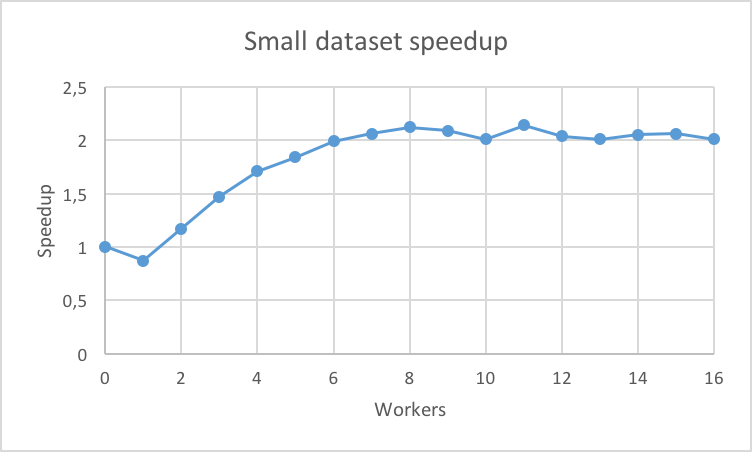
\includegraphics[width=120mm]{figures/dataset_2/dataset_2_speedup.png}
  \caption[Speedup plot for the small dataset.]{Speedup plot for the small dataset. The X axis shows the number of workers, and the Y axis shows a scalar value signifying the speedup as
  ``number of times faster than sequential execution''. Speedup increases with each worker, evening out around 8 workers and 2.1X speedup.}
  \label{fig:dataset_2_speedup}
\end{figure}

\subsection{Medium dataset speedup}
The speedup for the medium dataset can be found in figure \ref{fig:dataset_3_speedup}.
The X axis shows the number of workers, and the Y axis shows a scalar value signifying the speedup as
``number of times faster than sequential execution''. Speedup increases with each worker, evening out around 8-9 workers and 3.8X speedup.
\begin{figure}[ht]
  \centering
  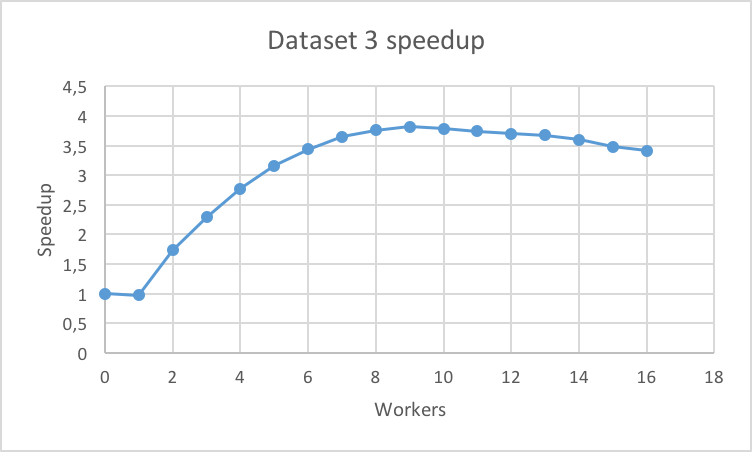
\includegraphics[width=120mm]{figures/dataset_3/dataset_3_speedup.png}
  \caption[Speedup plot for the medium dataset.]{Speedup plot for the medium dataset. The X axis shows the number of workers, and the Y axis shows a scalar value signifying the speedup as
  ``number of times faster than sequential execution''. Speedup increases with each worker, evening out around 8-9 workers and 3.8X speedup.}
  \label{fig:dataset_3_speedup}
\end{figure}

%\subsection{Large dataset speedup}
%The speedup for the large dataset can be found in figure \ref{fig:dataset_4_speedup}.
%The X axis shows the number of workers, and the Y axis shows a scalar value signifying the speedup as
%``number of times faster than sequential execution''. Speedup increases with each worker, evening out around 12 workers and 4.2X speedup.
%\begin{figure}[ht]
  %\centering
  %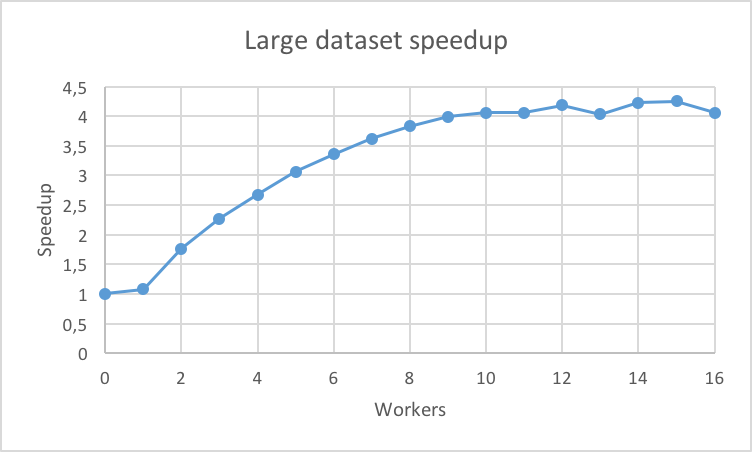
\includegraphics[width=120mm]{figures/dataset_4/dataset_4_speedup.png}
  %\caption[Speedup plot for the large dataset.]{Speedup plot for the large dataset. The X axis shows the number of workers, and the Y axis shows a scalar value signifying the speedup as
  %``number of times faster than sequential execution''. Speedup increases with each worker, evening out around 12 workers and 4.2X speedup.}
  %\label{fig:dataset_4_speedup}
%\end{figure}

\section{Memory consumption}

\subsection{Tiny dataset memory consumption}
The memory consumption for the tiny dataset can be found in figure \ref{fig:dataset_1_memory}.
The X axis shows the numner of workers, and the Y axis shows the total memory usage as
a sum of the highest memory usage for each worker process, in addition to the main process. Memory usage increases close to linearly with each added worker,
up to about 1.6 GB for 16 workers.
\begin{figure}[ht]
  \centering
  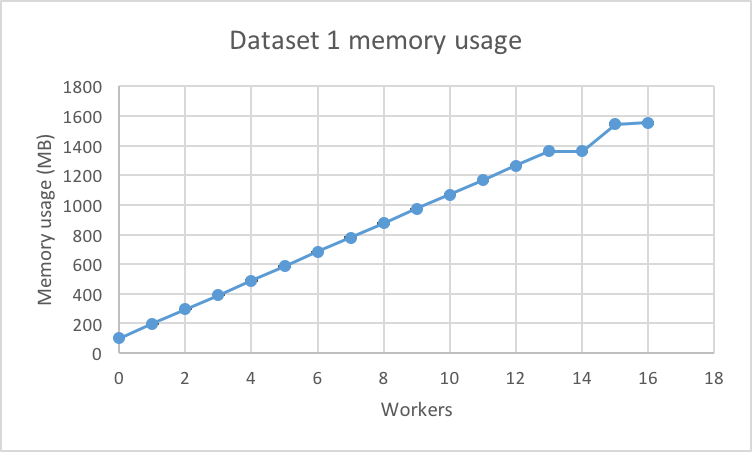
\includegraphics[width=120mm]{figures/dataset_1/dataset_1_memory.png}
  \caption[Memory usage plot for the tiny dataset.]{Memory usage plot for the tiny dataset. The X axis shows the numner of workers, and the Y axis shows the total memory usage as
  a sum of the highest memory usage for each worker process, in addition to the main process. Memory usage increases close to linearly with each added worker,
  up to about 1.6 GB for 16 workers.}
  \label{fig:dataset_1_memory}
\end{figure}

\subsection{Small dataset memory consumption}
The memory consumption for the tiny dataset can be found in figure \ref{fig:dataset_2_memory}.
The X axis shows the numner of workers, and the Y axis shows the total memory usage as
a sum of the highest memory usage for each worker process, in addition to the main process. Memory usage increases close to linearly with each added worker,
up to about 2 GB for 16 workers.
\begin{figure}[ht]
  \centering
  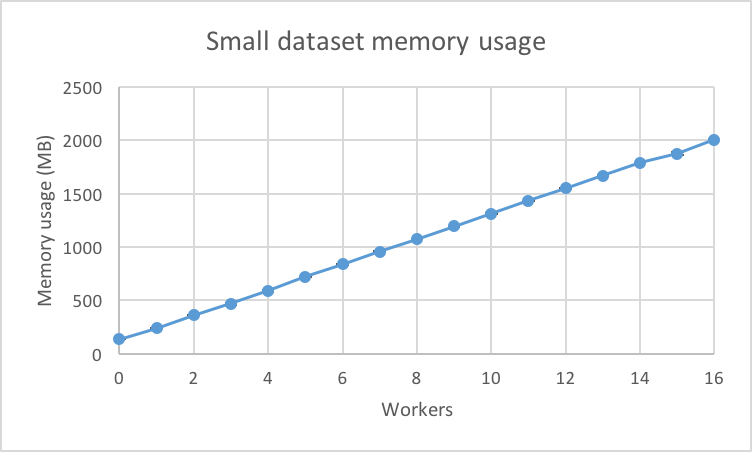
\includegraphics[width=120mm]{figures/dataset_2/dataset_2_memory.png}
  \caption[Memory usage plot for the small dataset.]{Memory usage plot for the small dataset. The X axis shows the numner of workers, and the Y axis shows the total memory usage as
  a sum of the highest memory usage for each worker process, in addition to the main process. Memory usage increases close to linearly with each added worker,
  up to about 2 GB for 16 workers.}
  \label{fig:dataset_2_memory}
\end{figure}

\subsection{Medium dataset memory consumption}
The memory consumption for the tiny dataset can be found in figure \ref{fig:dataset_3_memory}.
The X axis shows the numner of workers, and the Y axis shows the total memory usage as
a sum of the highest memory usage for each worker process, in addition to the main process. Memory usage increases close to linearly with each added worker,
up to about 6 GB for 16 workers.
\begin{figure}[ht]
  \centering
  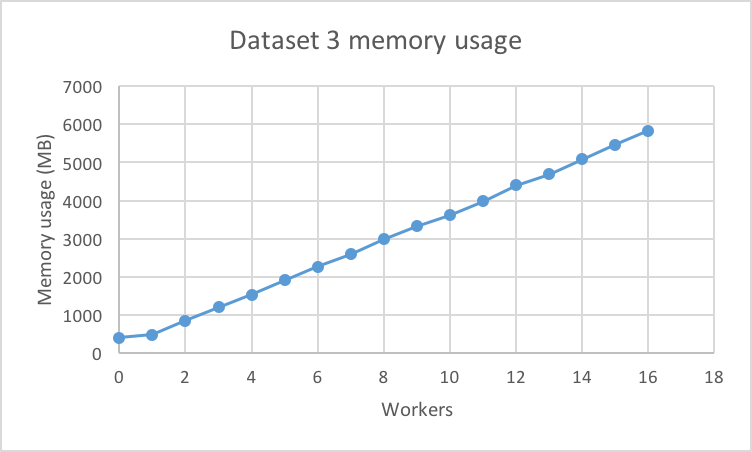
\includegraphics[width=120mm]{figures/dataset_3/dataset_3_memory.png}
  \caption[Memory usage plot for the medium dataset.]{Memory usage plot for the medium dataset. The X axis shows the numner of workers, and the Y axis shows the total memory usage as
  a sum of the highest memory usage for each worker process, in addition to the main process. Memory usage increases close to linearly with each added worker,
  up to about 6 GB for 16 workers.}
  \label{fig:dataset_3_memory}
\end{figure}

%\subsection{Large dataset memory consumption}
%The memory consumption for the tiny dataset can be found in figure \ref{fig:dataset_4_memory}.
%The X axis shows the numner of workers, and the Y axis shows the total memory usage as
%a sum of the highest memory usage for each worker process, in addition to the main process. Memory usage increases close to linearly with each added worker,
%up to about 8.8 GB for 16 workers.
%\begin{figure}[ht]
  %\centering
  %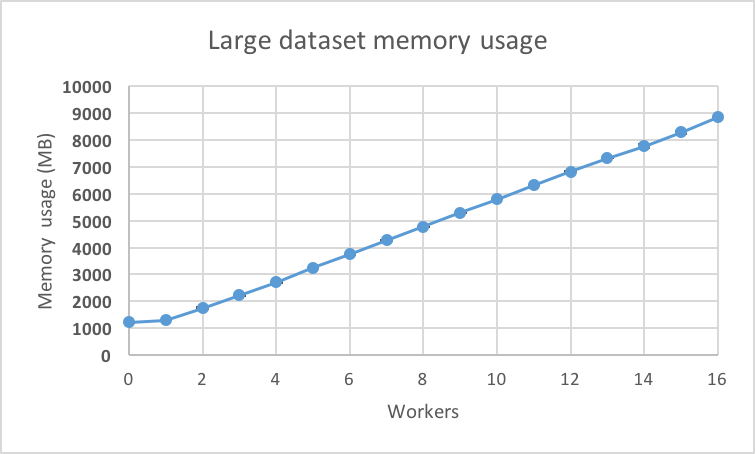
\includegraphics[width=120mm]{figures/dataset_4/dataset_4_memory.png}
  %\caption[Memory usage plot for the large dataset.]{Memory usage plot for the large dataset. The X axis shows the numner of workers, and the Y axis shows the total memory usage as
  %a sum of the highest memory usage for each worker process, in addition to the main process. Memory usage increases close to linearly with each added worker,
  %up to about 8.8 GB for 16 workers.}
  %\label{fig:dataset_4_memory}
%\end{figure}

\section{Parallel profiler analysis}
For each dataset, a profiling session of the parallel program was conducted. The same hardware as for the benchmarks was used, and
the profiling was done for a transformation run with 8 workers. The functions highlighted and discussed are the ones with the highest
cumulative time which are at the top level. These are the most interesting functions to examine as they take up a large part of the
running time, and other functions with high cumulative time are also called from these.

A function that is present in each of the analyses is \code{aggregate\_result}, which contains the code that creates the
other processes and waits for these to produce their partial results, aggregating them as they are produced. It is therefore a large
part of the execution time for each main process run. Another function seen in each main process is \code{post\_process\_parallel},
which is responsible for the sequential post processing step of making trade ID:s unique (which happens after \code{aggregate\_result}.

For the worker processes, \code{process} is the main dataset processing function, explaining its prominence in each profiling session.

\subsection{Tiny dataset profiler analysis}
The parallel program \code{cProfile} output for the tiny dataset can be found in figure \ref{fig:profiler_tiny_main} (main process)
and figure \ref{fig:profiler_tiny_worker} (worker process). Functions with low cumulative time have been omitted.

For the main process, the most prominent functions are \code{aggregate\_result} (70\% of the execution time), \code{perform\_header\_detection} (11.5\% of
the execution time), and \code{post\_process\_parallel} (7.8\% of the execution time).
\code{perform\_header\_detection} finds the header of the dataset, which the other processes needs to process their dataset chunks. 

For the worker process, apart from \code{process}, \code{readMessageBegin} (44.9\%) of the worker execution time
is one of the functions that take the most time. This function
is part of the communication protocol between the program and the database, indicating that communication takes up a large part of the
worker process for the tiny dataset, taking up larger portions of the total time than row processing functions such as \code{process\_record} (9.0\% of the execution time).

\begin{figure}[ht]
  \begin{VerbatimInput}{figures/dataset_1/dataset_1_profiling_main.txt}
    \caption[Parallel program \code{cProfile} output for the main process of the tiny dataset.]{Parallel program \code{cProfile} output for the main process of the tiny dataset.
    The most interesting functions are highlighted in green.
For the main process, the most prominent functions are \code{aggregate\_result} (70\% of the execution time), \code{perform\_header\_detection} (11.5\% of
the execution time), and \code{post\_process\_parallel} (7.8\% of the execution time).
  \code{perform\_header\_detection} finds the header of the dataset, which the other processes needs to process their dataset chunks.}
  \label{fig:profiler_tiny_main}
\end{VerbatimInput}
\end{figure}

\begin{figure}[ht]
  \begin{VerbatimInput}{figures/dataset_1/dataset_1_profiling_worker.txt}
    \caption[Parallel program \code{cProfile} output for a worker process of the tiny dataset.]{Parallel program \code{cProfile} output for a worker process of the tiny dataset.
    The most interesting functions are highlighted in green.
For the worker process, apart from \code{process}, \code{readMessageBegin} (44.9\%) of the worker execution time
is one of the functions that take the most time. This function
is part of the communication protocol between the program and the database, indicating that communication takes up a large part of the
worker process for the tiny dataset, taking up larger portions of the total time than row processing functions such as \code{process\_record} (9.0\% of the execution time).}
  \label{fig:profiler_tiny_worker}
\end{VerbatimInput}
\end{figure}

\subsection{Small dataset profiler analysis}
The parallel program \code{cProfile} output for the small dataset can be found in figure \ref{fig:profiler_small_main} (main process) and figure \ref{fig:profiler_small_worker}
(worker process). Functions with low cumulative time have been omitted.

For the main process, the major functions are \code{aggregate\_result} (71.7\%) and \code{post\_process\_parallel} (22.5\%).

For the worker process \code{\_fetch\_all} (38\%) is responisble for getting the dataset rows. The row processing functions take up a larger portion of the code
than for the tiny dataset, 33.6\% for \code{post\_process\_record}, 21.5\% for \code{consume\_record}, and 14.6\% for \code{process\_record}.

\begin{figure}[ht]
  \begin{VerbatimInput}{figures/dataset_2/dataset_2_profiling_main.txt}
    \caption[Parallel program \code{cProfile} output for the main process of the small dataset.]{Parallel program \code{cProfile} output for the main process of the small dataset.
    The most interesting functions are highlighted in green.
  For the main process, the major functions are \code{aggregate\_result} (71.7\%) and \code{post\_process\_parallel} (22.5\%).}
  \label{fig:profiler_small_main}
\end{VerbatimInput}
\end{figure}

\begin{figure}[ht]
  \begin{VerbatimInput}{figures/dataset_2/dataset_2_profiling_worker.txt}
    \caption[Parallel program \code{cProfile} output for a worker process of the small dataset.]{Parallel program \code{cProfile} output for a worker process of the small dataset.
    The most interesting functions are highlighted in green.
  For the worker process \code{\_fetch\_all} (38\%) is responisble for getting the dataset rows. The row processing functions take up a larger portion of the code
than for the tiny dataset, 33.6\% for \code{post\_process\_record}, 21.5\% for \code{consume\_record}, and 14.6\% for \code{process\_record}.}
  \label{fig:profiler_small_worker}
\end{VerbatimInput}
\end{figure}

\subsection{Medium dataset profiler analysis}
The parallel program \code{cProfile} output for the medium dataset can be found in figure \ref{fig:profiler_medium_main} (main process) and figure \ref{fig:profiler_medium_worker}
(worker process). Functions with low cumulative time have been omitted.

For the main process, the major functions are \code{aggregate\_result} (91.1\%) and \code{post\_process\_parallel} (7.0\%).

For the worker process, the functions related to row processing are more prominent: \code{process\_record} (26\%), \code{post\_process\_record} (24.8\%), \code{consume\_record}
(8.7\%). \code{\_prepare}, called before the main row processing loop, takes up 22\% of the total time.

\begin{figure}[ht]
  \begin{VerbatimInput}{figures/dataset_3/dataset_3_profiling_main.txt}
    \caption[Parallel program \code{cProfile} output for the main process of the medium dataset.]{Parallel program \code{cProfile} output for the main process of the medium dataset.
    The most interesting functions are highlighted in green.
For the main process, the major functions are \code{aggregate\_result} (91.1\%) and \code{post\_process\_parallel} (7.0\%).}
  \label{fig:profiler_medium_main}
\end{VerbatimInput}
\end{figure}

\begin{figure}[ht]
  \begin{VerbatimInput}{figures/dataset_3/dataset_3_profiling_worker.txt}
    \caption[Parallel program \code{cProfile} output for a worker process of the medium dataset.]{Parallel program \code{cProfile} output for a worker process of the medium dataset.
    The most interesting functions are highlighted in green.
For the worker process, the functions related to row processing are more prominent: \code{process\_record} (26\%), \code{post\_process\_record} (24.8\%), \code{consume\_record}
(8.7\%). \code{\_prepare}, called before the main row processing loop, takes up 22\% of the total time.}
  \label{fig:profiler_medium_worker}
\end{VerbatimInput}
\end{figure}

\section{Performance without sequential post processing}
As the sequential profiling adds overhead, it is interesting to see what the speedup would have been if this extra step was not needed.
These results are based in the profiling session above, conducted with 8 workers.

For the tiny dataset, the post processing adds 7.8\% overhead. Subtracting 7.8\% percent from the run with 8 workers results in a decrease
from 1.74 s to 1.6 s. This means the ``speedup'' goes from 0.6X to 0.69X.

For the small dataset, the post processing adds 22\% overhead. Subtracting 22\% percent from the run with 8 workers results in a decrease
from 7.21 s to 5.62 s. This means the speedup goes from 2.11X to 2.72X.

For the medium dataset, the post processing adds 7\% overhead. Subtracting 7\% percent from the run with 8 workers results in a decrease

from 19.94 s to 18.54 s. This means the speedup goes from 3.76X to 4.04X.

\section{Targeted memory profiling}
In order to find the source of memory overhead, a simple targeted memory profiling was conducted by finding (using \code{resource}) and
printing the current highest memory usage before and after some of the major functions in the program.
